\documentclass[a4paper, 12pt]{extreport}

\usepackage[T2A]{fontenc}
\usepackage[utf8]{inputenc}
\usepackage[english,russian]{babel}
\usepackage{amssymb,amsfonts,amsmath,mathtext,cite,enumerate,float}
\usepackage{pgfplots}
\usepackage{graphicx}
\usepackage{tocloft}
\usepackage{listings}
\usepackage{caption}
\usepackage{tempora}
\usepackage{titlesec}
\usepackage{setspace}
\usepackage{geometry}
\usepackage{indentfirst}
\documentclass{article}
\usepackage{pdfpages}
\usepackage{enumerate,letltxmacro}
\usepackage{threeparttable}
\usepackage[hidelinks]{hyperref}
\usepackage{flafter}
\usepackage{enumitem}
\usepackage{multirow}

\usepackage[figure,table]{totalcount}
\usepackage{lastpage}

\setlist{nosep}

\newcommand{\ssr}[1]{\begin{center}
		\LARGE\bfseries{#1}
	\end{center} \addcontentsline{toc}{chapter}{#1}  }

\makeatletter
\renewcommand\LARGE{\@setfontsize\LARGE{22pt}{20}}
\renewcommand\Large{\@setfontsize\Large{20pt}{20}}
\renewcommand\large{\@setfontsize\large{16pt}{20}}
\makeatother
\RequirePackage{titlesec}
\titleformat{\chapter}[block]{\hspace{\parindent}\large\bfseries}{\thechapter}{0.5em}{\large\bfseries\raggedright}
\titleformat{name=\chapter,numberless}[block]{\hspace{\parindent}}{}{0pt}{\large\bfseries\centering}
\titleformat{\section}[block]{\hspace{\parindent}\large\bfseries}{\thesection}{0.5em}{\large\bfseries\raggedright}
\titleformat{\subsection}[block]{\hspace{\parindent}\large\bfseries}{\thesubsection}{0.5em}{\large\bfseries\raggedright}
\titleformat{\subsubsection}[block]{\hspace{\parindent}\large\bfseries}{\thesubsection}{0.5em}{\large\bfseries\raggedright}
\titlespacing{\chapter}{12.5mm}{-22pt}{10pt}
\titlespacing{\section}{12.5mm}{10pt}{10pt}
\titlespacing{\subsection}{12.5mm}{10pt}{10pt}
\titlespacing{\subsubsection}{12.5mm}{10pt}{10pt}

\makeatletter
\renewcommand{\@biblabel}[1]{#1.}
\makeatother
%
%\titleformat{\chapter}[hang]{\LARGE\bfseries}{\hspace{1.25cm}\thechapter}{1ex}{\LARGE\bfseries}
%\titleformat{\section}[hang]{\Large\bfseries}{\hspace{1.25cm}\thesection}{1ex}{\Large\bfseries}
%\titleformat{name=\section,numberless}[hang]{\Large\bfseries}{\hspace{1.25cm}}{0pt}{\Large\bfseries}
%\titleformat{\subsection}[hang]{\large\bfseries}{\hspace{1.25cm}\thesubsection}{1ex}{\large\bfseries}
%\titlespacing{\chapter}{0pt}{-\baselineskip}{\baselineskip}
%\titlespacing*{\section}{0pt}{\baselineskip}{\baselineskip}
%\titlespacing*{\subsection}{0pt}{\baselineskip}{\baselineskip}

\geometry{left=30mm}
\geometry{right=10mm}
\geometry{top=20mm}
\geometry{bottom=20mm}

\onehalfspacing

\renewcommand{\theenumi}{\arabic{enumi}}
\renewcommand{\labelenumi}{\arabic{enumi}\text{)}}
\renewcommand{\theenumii}{.\arabic{enumii}}
\renewcommand{\labelenumii}{\asbuk{enumii}\text{)}}
\renewcommand{\theenumiii}{.\arabic{enumiii}}
\renewcommand{\labelenumiii}{\arabic{enumi}.\arabic{enumii}.\arabic{enumiii}.}

\renewcommand{\cftchapleader}{\cftdotfill{\cftdotsep}}

\addto\captionsrussian{\renewcommand{\figurename}{Рисунок}}
\DeclareCaptionLabelSeparator{dash}{~---~}
\captionsetup{labelsep=dash}

\captionsetup[figure]{justification=centering,labelsep=dash}
\captionsetup[table]{labelsep=dash,justification=raggedright,singlelinecheck=off}

\graphicspath{{images/}}%путь к рисункам

\newcommand{\floor}[1]{\lfloor #1 \rfloor}

\lstset{ %
	language=caml,                 % выбор языка для подсветки (здесь это С)
	basicstyle=\small\ttfamily, % размер и начертание шрифта для подсветки кода
	numbers=none,               % где поставить нумерацию строк (слева\справа)
	numberstyle=\tiny,           % размер шрифта для номеров строк
	stepnumber=1,                   % размер шага между двумя номерами строк
%	numbersep=5pt,                % как далеко отстоят номера строк от подсвечиваемого кода
	showspaces=false,            % показывать или нет пробелы специальными отступами
	showstringspaces=false,      % показывать или нет пробелы в строках
	showtabs=false,             % показывать или нет табуляцию в строках
	frame=single,              % рисовать рамку вокруг кода
	tabsize=2,                 % размер табуляции по умолчанию равен 2 пробелам
	captionpos=t,              % позиция заголовка вверху [t] или внизу [b] 
	breaklines=true,           % автоматически переносить строки (да\нет)
	breakatwhitespace=false, % переносить строки только если есть пробел
	escapeinside={\#*}{*)},   % если нужно добавить комментарии в коде
	abovecaptionskip=-5pt
}

\pgfplotsset{width=0.85\linewidth, height=0.5\columnwidth}

\linespread{1.3}

\parindent=1.25cm

%\LetLtxMacro\itemold\item
%\renewcommand{\item}{\itemindent0.75cm\itemold}

\def\labelitemi{---}
\setlist[itemize]{leftmargin=1.25cm, itemindent=0.65cm}
\setlist[enumerate]{leftmargin=1.25cm, itemindent=0.55cm}

\newcommand{\specialcell}[2][c]{%
	\begin{tabular}[#1]{@{}c@{}}#2\end{tabular}}

\frenchspacing


\begin{document}
\begin{titlepage}
	\newgeometry{pdftex, left=2cm, right=2cm, top=2.5cm, bottom=2.5cm}
	\fontsize{12pt}{12pt}\selectfont
	\noindent \begin{minipage}{0.15\textwidth}
		
\includegraphics[width=\linewidth]{img/b_logo.png}
	\end{minipage}
	\noindent\begin{minipage}{0.9\textwidth}\centering
		\textbf{Министерство науки и высшего образования Российской Федерации}\\
		\textbf{Федеральное государственное бюджетное образовательное учреждение высшего образования}\\
		\textbf{«Московский государственный технический университет имени Н. Э.~Баумана}\\
		\textbf{(национальный исследовательский университет)»}\\
		\textbf{(МГТУ им. Н. Э.~Баумана)}
	\end{minipage}

	\noindent\rule{18cm}{3pt}
	\newline\newline
	\noindent ФАКУЛЬТЕТ $\underline{\text{«Информатика и системы управления»~~~~~~~~~~~~~~~~~~~~~~~~~~~~~~~~~~~~~~~~~~~~~~~~~~~~~~~}}$ \newline\newline
	\noindent КАФЕДРА $\underline{\text{«Программное обеспечение ЭВМ и информационные технологии»~~~~~~~~~~~~~~~~~~~~~~~}}$\newline\newline\newline\newline\newline\newline\newline

	\begin{center}
		\noindent\begin{minipage}{1.3\textwidth}\centering
		\Large\textbf{   ~~~ Лабораторная работа №1}\newline
		\textbf{по дисциплине <<Анализ Алгоритмов>>}\newline\newline\newline
		\end{minipage}
	\end{center}

	\noindent\textbf{Тема} 			$\underline{\text{Расстояние Левенштейна и Дамерау~---~Левенштейна}}$\newline\newline
	\noindent\textbf{Студент} 		$\underline{\text{Платонова М. И.}}$\newline\newline
	\noindent\textbf{Группа} 		$\underline{\text{ИУ7-51Б}}$\newline\newline
	\noindent\textbf{Преподаватель} $\underline{\text{Волкова Л. Л.}}$\newline

	\begin{center}
		\vfill
		Москва~---~\the\year
		~г.
	\end{center}
	\restoregeometry
\end{titlepage}

\def\contentsname{\begin{center}\MakeUppercase{СОДЕРЖАНИЕ}\end{center}}
\tableofcontents
\setcounter{page}{2}

\chapter*{ВВЕДЕНИЕ}
\addcontentsline{toc}{chapter}{ВВЕДЕНИЕ}
В данной лабораторной работе будет исследовано расстояние Левенштейна, которое представляет собой минимальное количество операций, требуемых для преобразования одной строки в другую. К таким операциям относятся вставка, удаление и замена символов. Расстояние Левенштейна используется для оценки различий между строками.

Применение расстояния Левенштейна возможно в различных областях:
\begin{itemize}
    \item[--] корректировка опечаток и ошибок при наборе текста для повышения удобства ввода данных;
    \item[--] анализ изменений в текстовых файлах, что полезно при работе с системами управления версиями;
    \item[--] оптимизация поиска схожих строк в больших текстах, используется в поисковых системах.
\end{itemize}

Целью данной лабораторной работы является исследование и реализация алгоритмов для вычисления расстояния Левенштейна, а также его модификации~---~Дамерау~---~Левенштейна. 
Для достижения этой цели необходимо выполнить следующие задачи:

\begin{itemize}
    \item[--] исследовать методы расчёта расстояния Левенштейна и Дамерау~---~Левенштейна;
    \item[--] реализовать рекурсивный алгоритм для вычисления расстояния Левенштейна;
    \item[--] реализовать нерекурсивный алгоритм для вычисления расстояния Левенштейна;
    \item[--] реализовать рекурсивный с кэшем алгоритм для вычисления расстояния Левенштейна;
    \item[--] реализовать рекурсивный алгоритм для вычисления расстояния Дамерау~---~Левенштейна;
    \item[--] провести сравнение эффективности этих алгоритмов, исследуя их затраты по затраченному процессорному времени и памяти;
    \item[--] сформулировать и представить результаты в отчёте о проведённой лабораторной работе.
\end{itemize}


\chapter{Аналитическая часть}
В данном разделе будут рассмотрены алгоритмы нахождения расстояний Левенштейна и Дамерау~---~Левенштейна.
\section{Расстояние Левенштейна}

Расстояние Левенштейна [1] --- это минимальное количество операций вставки, удаления и замены, необходимых для превращения одной строки в другую.

Каждая из редакторских операций обладает определённой стоимостью (штрафом), которая может изменяться в зависимости от контекста и требований. В данной работе рассматриваются алгоритмы, для которых стоимость всех операций равна 1. Такой подход упрощает анализ и сравнение различных алгоритмов. 
\begin{itemize}
        \item[--] $w(\lambda, \lambda) = 0$ --- между пустыми символами ($\lambda$ обозначает пустую строку);
	\item[--] $w(a, b) = 1$ --- цена замены символа $a$ на $b$, R (от англ. replace);
	\item[--] $w(\lambda, b) = 1$ --- цена вставки символа $b$, I (от англ. insert);
	\item[--] $w(a, \lambda) = 1$ --- цена удаления символа $a$, D (от англ. delete).
\end{itemize}

Пусть $x, y, z$ — это произвольные символы. Значит, операции, применимые к строкам, состоящим из этих символов, могут быть представлены следующим образом:
\begin{itemize}
    \item[--] вставка символа: $xy \rightarrow xyz$;
    \item[--] удаление символа: $xyz \rightarrow xy$;
    \item[--] замена символа: $dog \rightarrow log$.
\end{itemize}

\section{Формула вычисления расстояния Левенштейна}
Имеются две строки $S_{1}$ и $S_{2}$, длины $m$ и $n$ соответственно. Расстояние Левенштейна определяется с помощью рекуррентной формулы~(\ref{eq:L}):

\begin{equation}
	\label{eq:L}
	D(i, j) = \begin{cases}
	0, &\text{i = 0, j = 0}\\
	i, &\text{j = 0, i > 0}\\
	j, &\text{i = 0, j > 0}\\
	min \begin{cases}
		D(i, j - 1) + 1\\
		D(i - 1, j) + 1\\
		D(i - 1, j - 1), \text{если $S_{1}[i]= S_{2}[j]$} \\
            D(i - 1, j - 1) + 1, \text{если $S_{1}[i] \neq S_{2}[j]$} \\
	\end{cases}
	&\text{i > 0, j > 0}
	\end{cases}
\end{equation}

Таким образом, можно последовательно заполнить матрицу, где каждое значение в ячейках с индексами $i$ и $j$ отражает расстояние Левенштейна между подстроками $S_{1}[:i]$ и $S_{2}[:j]$. Итоговое значение расстояния Левенштейна для строк $S_{1}$ и $S_{2}$ будет расположено в ячейке $D(m, n)$.


\section{Расстояние Дамерау~---~Левенштейна}
Расстояние Дамерау~---~Левенштейна определяется как минимальное количество редакторских операций, необходимых для преобразования одной строки в другую. В дополнение к операциям вставки, удаления и замены, здесь также учитывается операция транспозиции, которая позволяет менять местами две соседние буквы, например, $\text{метр}\rightarrow \text{мерт}$.


\section{Формула вычисления расстояния Дамерау~---~Левенштейна}

Имеются две строки $S_{1}$ и $S_{2}$, длины $m$ и $n$ соответственно. Расстояние Дамерау~---~Левенштейна рассчитывается по следующей рекуррентной формуле~(\ref{eq:DL}):

\begin{equation}
	\label{eq:DL}
	D(i, j) = \begin{cases}
	0, \qquad\qquad\qquad\qquad\qquad\qquad\qquad\quad  j = 0, i = 0\\
	i, \qquad\qquad\qquad\qquad\qquad\qquad\qquad\quad  i = 0, i > 0\\
	j,\qquad\qquad\qquad\qquad\qquad\qquad\qquad\quad j > 0, i = 0\\
	min \begin{cases}
		D(i, j - 1) + 1,\\
		D(i - 1, j) + 1,\\
		D(i - 1, j - 1),\\\qquad\qquad\text{если $S_{1}[i]= S_{2}[j]$}, \\
            D(i - 1, j - 1) + 1,\\\qquad\qquad\text{если $S_{1}[i] \neq S_{2}[j]$}, \\
		D(i - 2, j - 2),\\\qquad\qquad\text{если $S_{1}[i]= S_{2}[j]$}, \\
            D(i - 2, j - 2) + 1,\\\qquad\qquad\text{если $S_{1}[i] \neq S_{2}[j]$}, \\
	\end{cases}
	\begin{aligned}
		& \text{если i > 1, j > 1} \\
		& S_{1}[i] = S_{2}[j - 1]  \\
		& S_{1}[j] =  S_{2}[i - 1] \\
	\end{aligned}\\
	min \begin{cases}
		D(i, j - 1) + 1,\\
		D(i - 1, j) + 1, & \;\; \text{иначе}\\
		D(i - 1, j - 1),\\\qquad\qquad\text{если $S_{1}[i]= S_{2}[j]$}, \\
            D(i - 1, j - 1) + 1,\\\qquad\qquad\text{если $S_{1}[i] \neq S_{2}[j]$}, \\
	\end{cases}
	\end{cases}
\end{equation}
\newline

В результате выполнения поэтапного заполнения матрицы каждая ячейка с координатами $i$ и $j$ будет содержать значение расстояния Дамерау~---~Левенштейна для подстрок $S_{1}[:i]$ и $S_{2}[:j]$.Итоговое значение расстояния Дамерау~---~Левенштейна для строк $S_{1}$ и $S_{2}$ будет расположено в ячейке $D(m, n)$.

\section*{Вывод}
В данном разделе были рассмотрены расстояния Левенштейна и Дамерау~---~Левенштейна. Для вычисления этих расстояний представлены формулы, которые могут быть реализованы как рекурсивными, так и нерекурсивными алгоритмами.


\chapter{Конструкторская часть}
В данном разделе будут представлены схемы алгоритмов для вычисления расстояний Левенштейна и Дамерау~---~Левенштейна.

\section{Разработка схем алгоритмов}

На вход алгоритмов поступают строки $S_{1}$ и $S_{2}$, включающие как русские, так и английские буквы. Результатом работы алгоритмов является целое число, соответствующее искомому расстоянию.
Рисунки~\ref{fig:lev_matr}~---~\ref{fig:dam_lev} представляют схемы рекурсивных и нерекурсивных алгоритмов для вычисления расстояний Левенштейна и Дамерау~---~Левенштейна.
\clearpage

\begin{figure}[h]
    \centering
    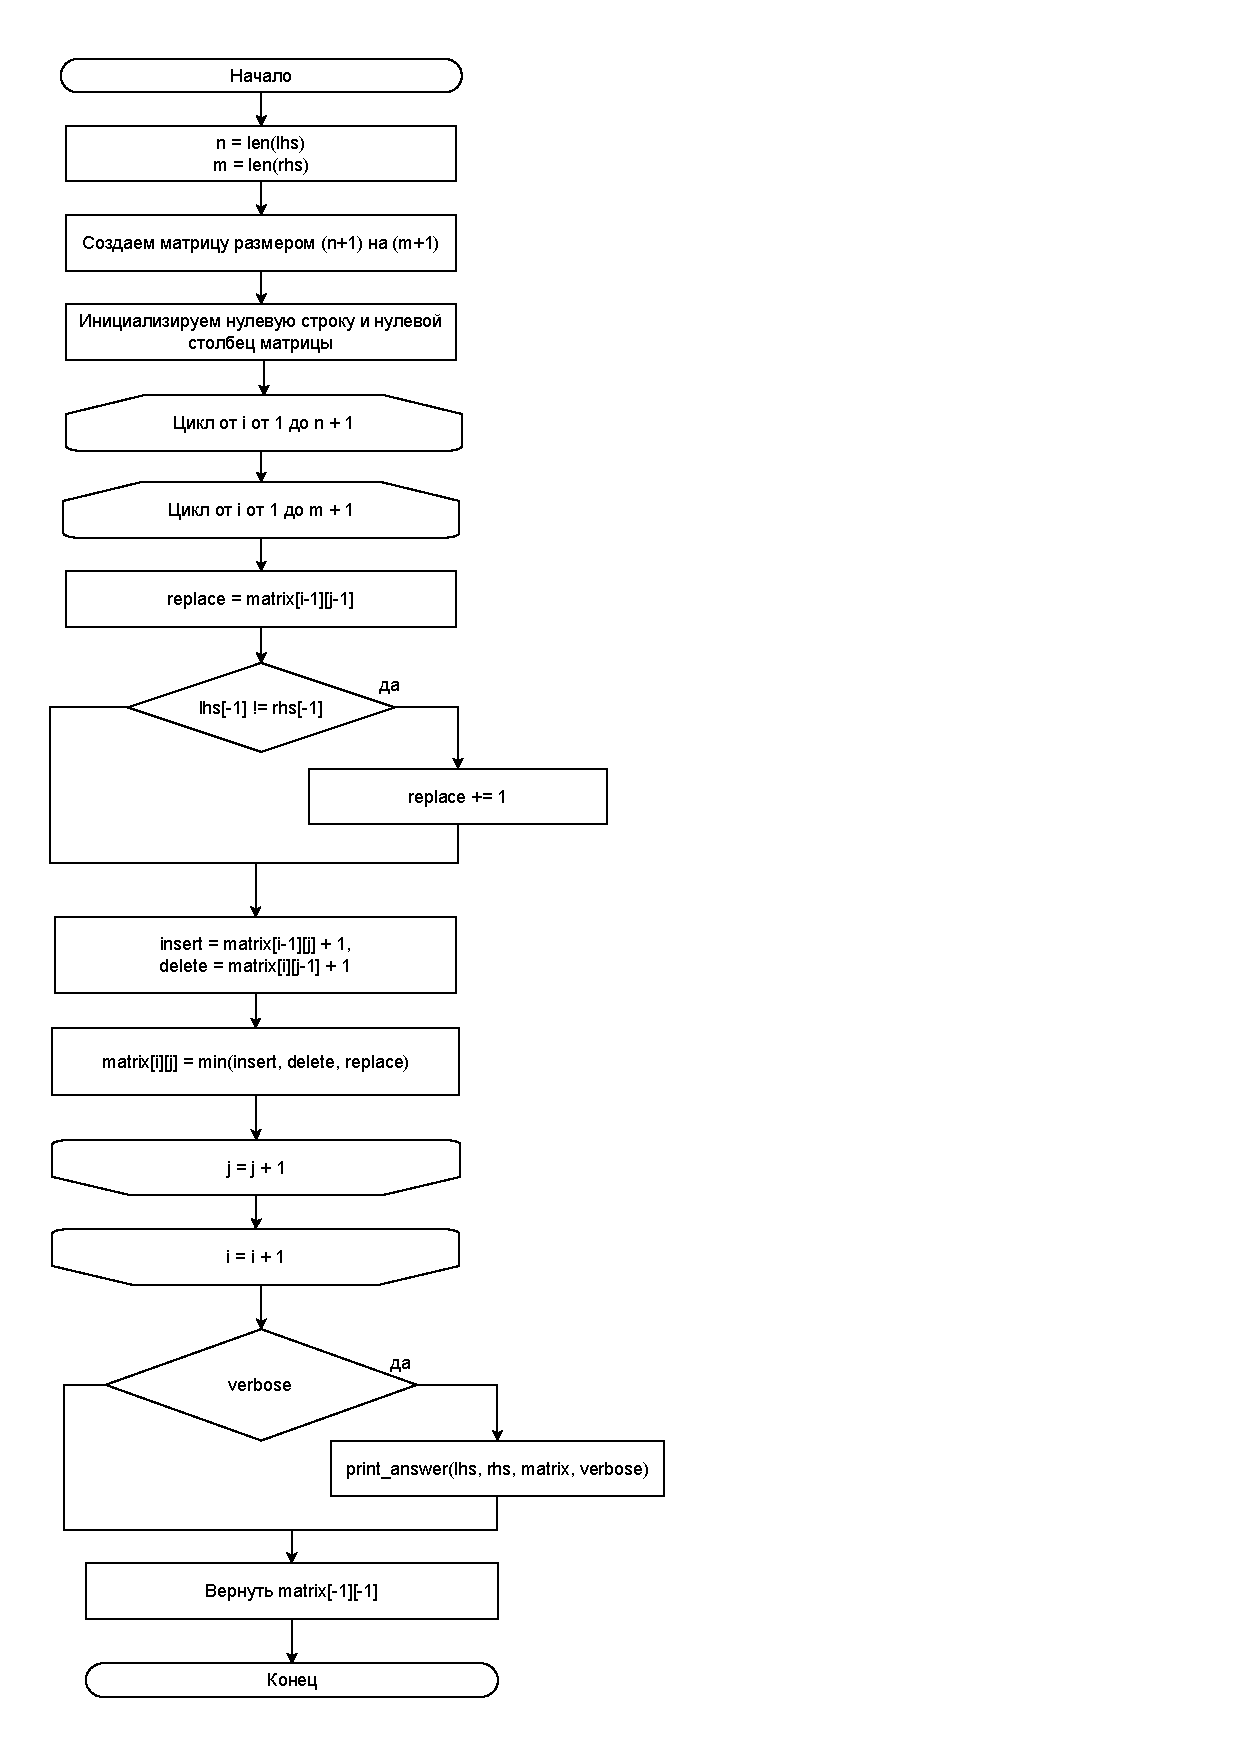
\includepdf[pages=1, scale=0.8, offset=5cm 0cm]{img/lev_matr.pdf} 
    \caption{Нерекурсивный алгоритм нахождения расстояния Левенштейна}
    \label{fig:lev_matr}
\end{figure}

\clearpage

\begin{figure}[h]
	\centering
	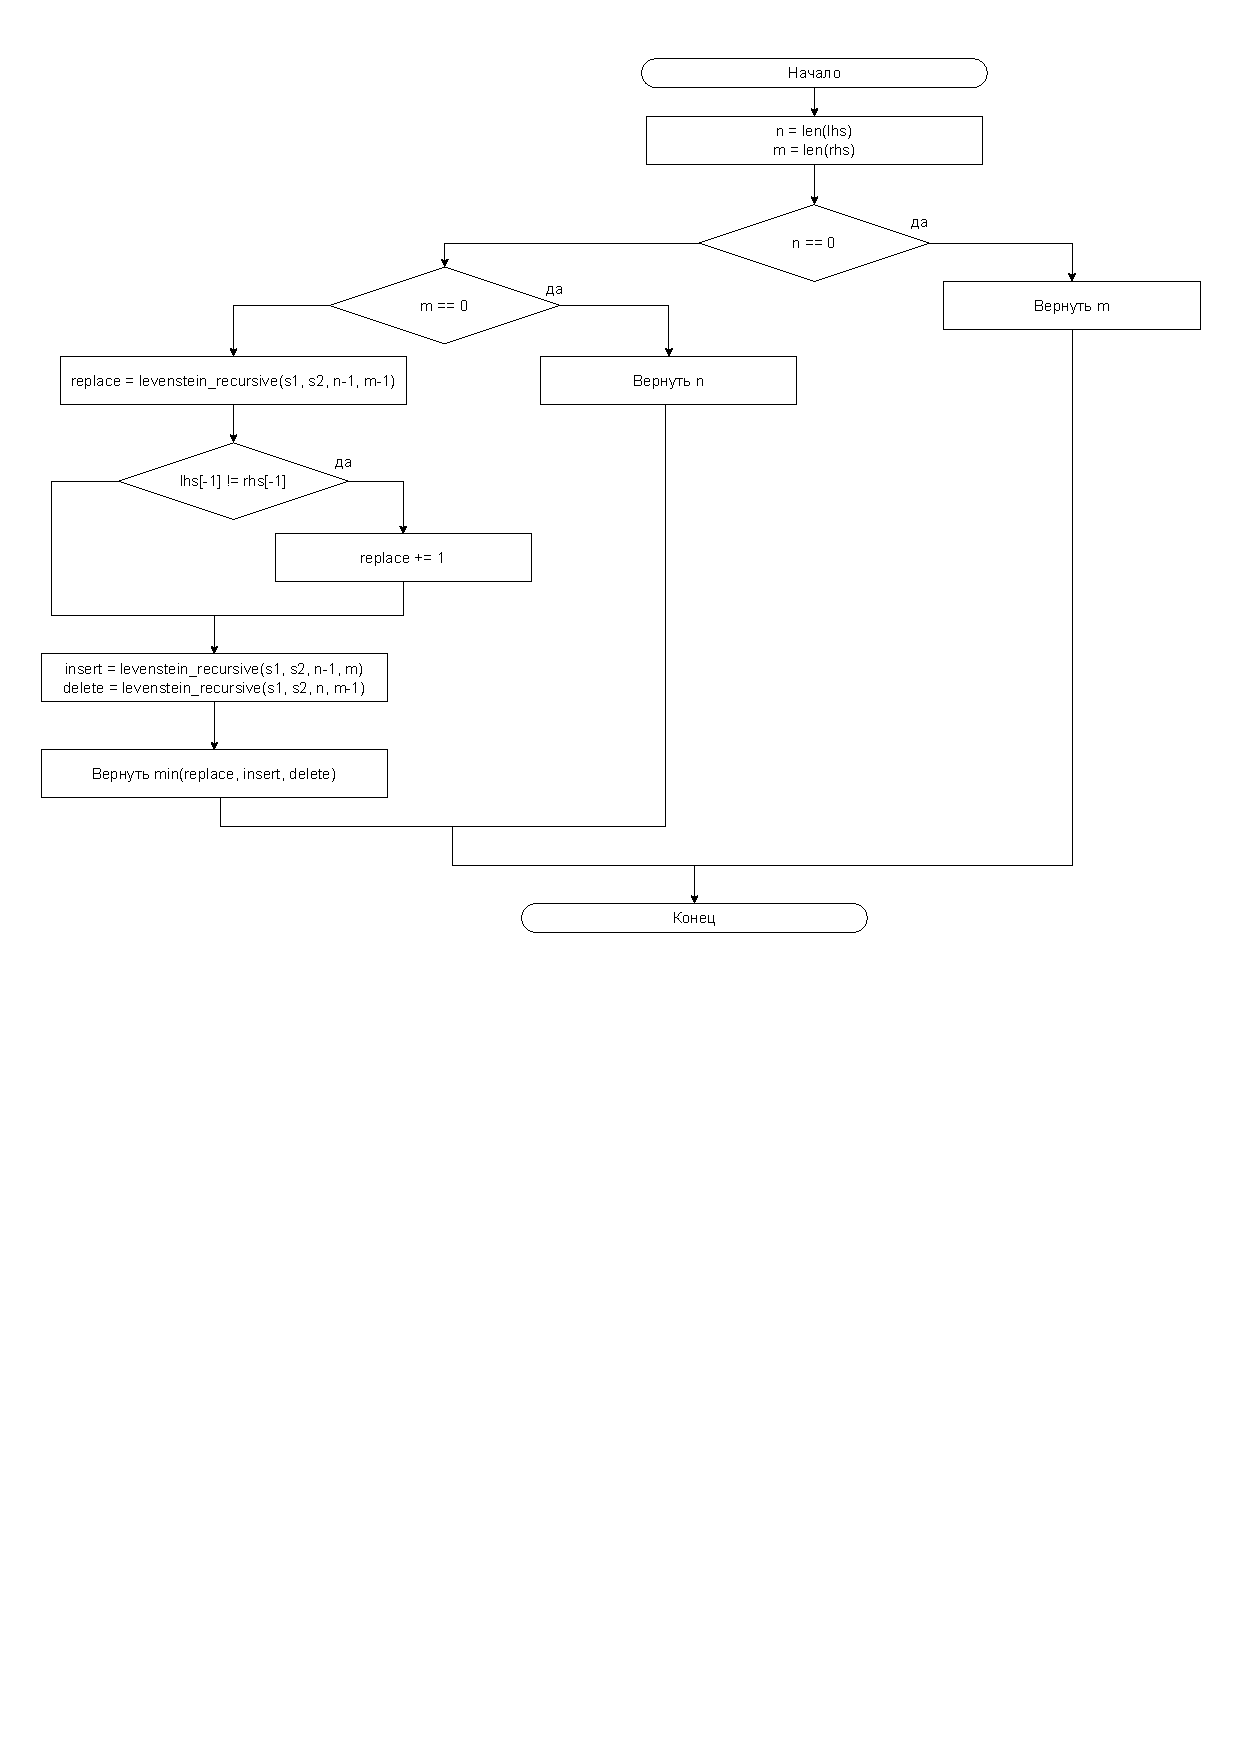
\includepdf[pages=1, scale=0.8]{img/lev_rec.pdf}
	\caption{Рекурсивный алгоритм нахождения расстояния Левенштейна}
	\label{fig:lev_rec}
\end{figure}

\clearpage  

\begin{figure}[h]
	\centering
	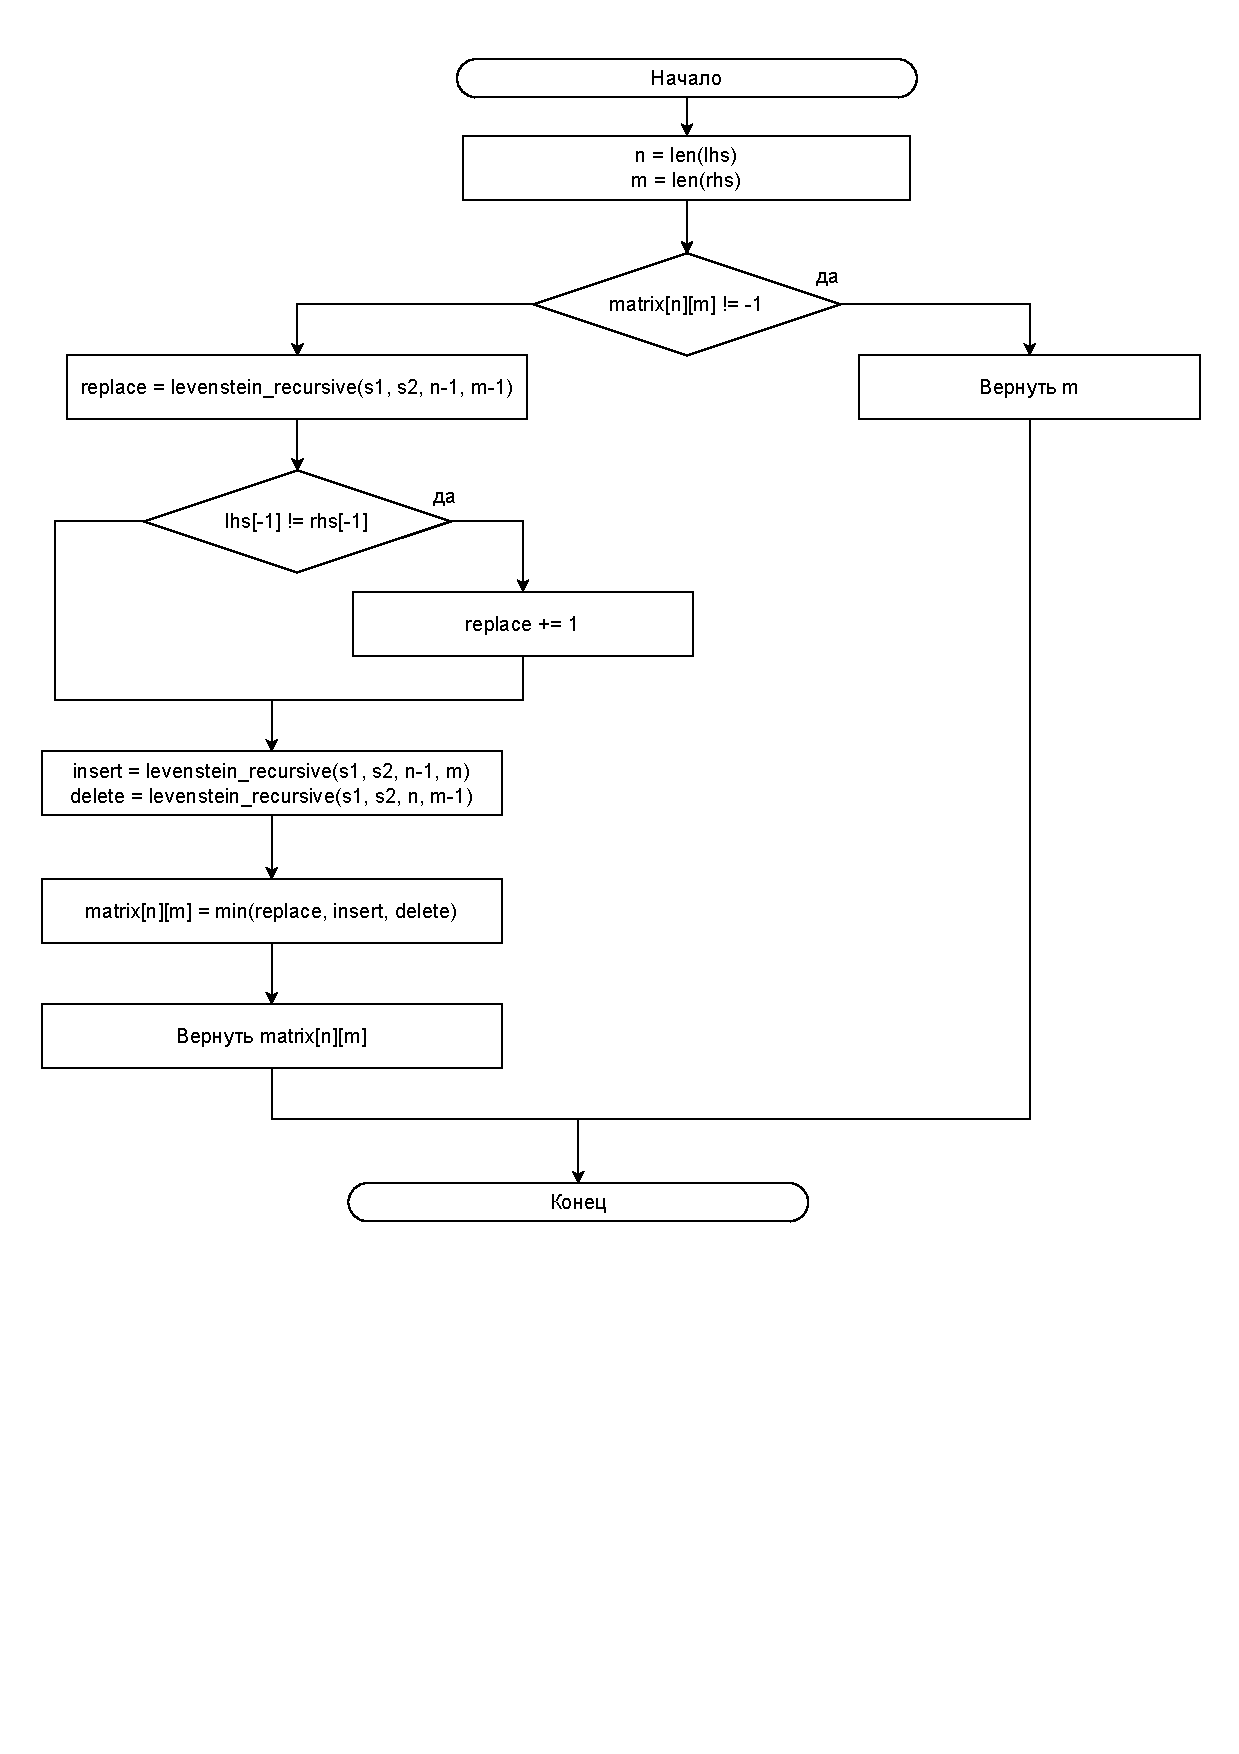
\includepdf[pages=1, scale=0.8]{img/lev_rec_cache.pdf}
	\caption{Рекурсивный алгоритм с кэшем нахождения расстояния Левенштейна}
	\label{fig:lev_rec_cache}
\end{figure}

\clearpage

\begin{figure}[h]
    \centering
    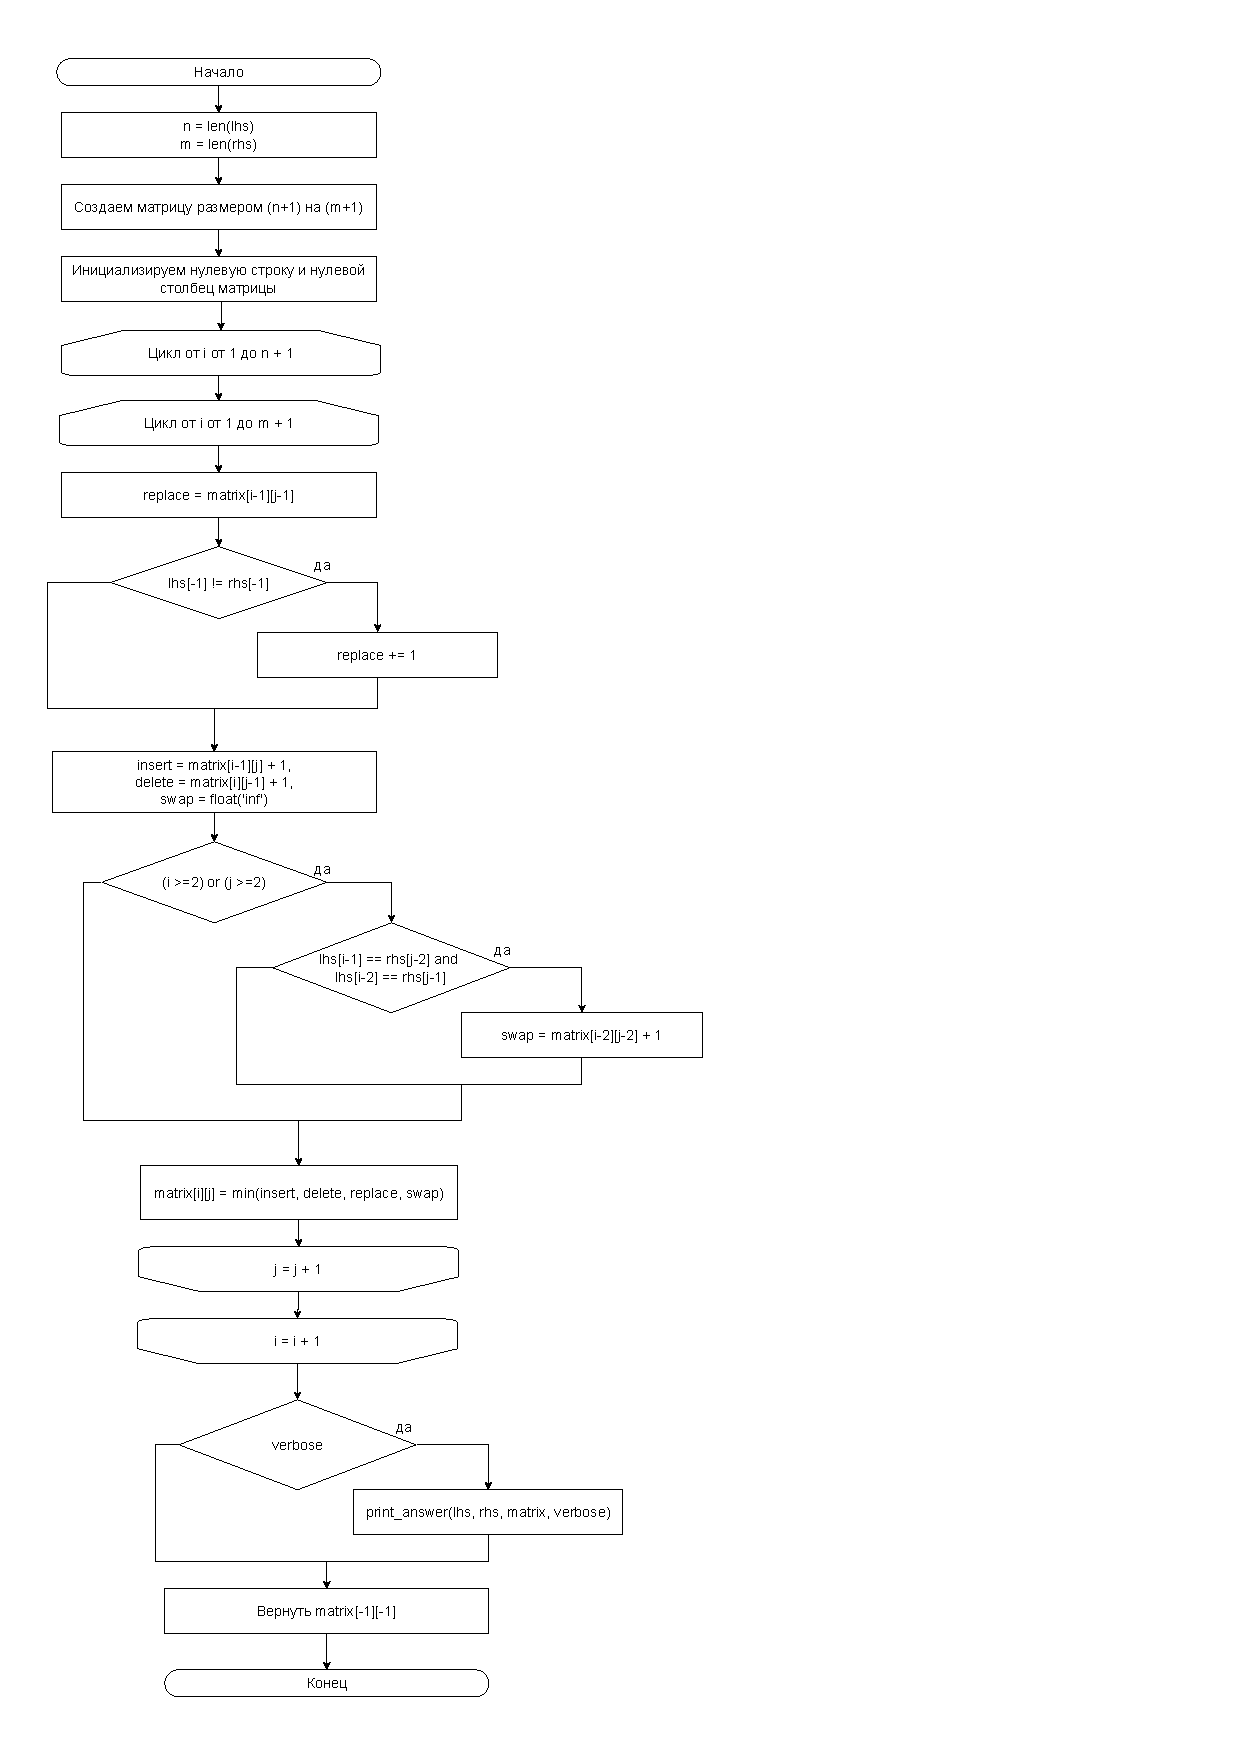
\includepdf[pages=1, scale=0.8, offset=5cm 0cm]{img/dam_lev.pdf}
    \caption{Нерекурсивный алгоритм нахождения расстояния Дамерау~---~Левенштейна}
    \label{fig:dam_lev}
\end{figure}

\clearpage



\section*{Вывод}
В данном разделе были разработаны алгоритмы для нерекурсивного, рекурсивного и рекурсивного с кэшем поиска расстояния Левенштейна, а также нерекурсивного алгоритма поиска расстояния Дамерау~---~Левенштейна.
\clearpage


\chapter{Технологическая часть}
В данном разделе будут приведены данные о выбранном языке программирования, листинги кода и тесты для каждого алгоритма.
\section{Средства реализации}
В данной работе для реализации был выбран язык программирования \texttt{Python}~\cite{bib2}. Выбор обусловлен наличием компилятора \texttt{MicroPython}, который позволяет создавать программы для работы с микроконтроллером. 
Также язык включает в себя модуль \texttt{time}~\cite{bib3}, который предоставляет метод, позволяющий получать процессорное время в тактовых циклах. 

\section{Листинги кода}
\begin{center}
\captionsetup{justification=raggedright,singlelinecheck=off}
\begin{lstlisting}[label=lst:create_matrix,caption=Реализация создания матрицы для расстояния Левенштейна]
def create_matrix(n: int, m: int):
    matrix = [[0 for _ in range(m)] for _ in range(n)]
    for i in range(n):
        for j in range(m):
            if i == 0:
                matrix[i][j] = j
            elif j == 0:
                matrix[i][j] = i
            else:
                matrix[i][j] = -1
    return matrix
\end{lstlisting}
\end{center}


\begin{center}
\captionsetup{justification=raggedright,singlelinecheck=off}
\begin{lstlisting}[label=lst:print_answer,caption=Реализация вывода матрицы расстояний]
def print_answer(lhs: str, rhs: str, matrix, verbose=True):
    if not verbose:
        return  

    print("   " + "  ".join(f"{ch}" for ch in rhs))  
    
    for i, row in enumerate(matrix):
        if i == 0:
            print("  " + " ".join(f"{val:2}" for val in row))  
        else:
            print(f"{lhs[i - 1]} " + " ".join(f"{val:2}" for val in row)) 
\end{lstlisting}
\end{center}

\clearpage

\begin{center}
\captionsetup{justification=raggedright,singlelinecheck=off}
\begin{lstlisting}[label=lst:levenstein_matrix,caption=Реализация матричного нахождения расстояния Левенштейна]
def levenstein_matrix(lhs: str, rhs: str, verbose=False):
    n = len(lhs)
    m = len(rhs)

    matrix = create_matrix(n + 1, m + 1)

    for i in range(1, n + 1):
        for j in range(1, m + 1):
            replace = matrix[i - 1][j - 1]
            if lhs[i - 1] != rhs[j - 1]:
                replace += 1
            insert = matrix[i - 1][j] + 1
            delete = matrix[i][j - 1] + 1
        
            matrix[i][j] = min(insert, delete, replace)

    if verbose:
        print_answer(lhs, rhs, matrix, verbose)  

    return matrix[-1][-1]
\end{lstlisting}
\end{center}


\begin{center}
\captionsetup{justification=raggedright,singlelinecheck=off}
\begin{lstlisting}[label=lst:levenstein_recursive,caption=Реализация рекурсивного нахождения расстояния Левенштейна]
def levenstein_recursive(lhs: str, rhs: str):
    n = len(lhs)
    m = len(rhs)

    if n == 0:
        return m
    if m == 0:
        return n

    replace = levenstein_recursive(lhs[:-1], rhs[:-1])
    
    if lhs[-1] != rhs[-1]:
        replace += 1

    insert = levenstein_recursive(lhs[:-1], rhs) + 1
    delete = levenstein_recursive(lhs, rhs[:-1]) + 1

    return min(replace, insert, delete)
\end{lstlisting}
\end{center}

\clearpage

\begin{center}
\captionsetup{justification=raggedright,singlelinecheck=off}
\begin{lstlisting}[label=lst:levenstein_recursive_cash,caption=Реализация рекурсивного нахождения расстояния Левенштейна с кэшированием]
def levenstein_recursive_cash(lhs: str, rhs: str, matrix):
    n = len(lhs)
    m = len(rhs)
    if matrix[n][m] != -1:
        return matrix[n][m]
    
    replace = levenstein_recursive_cash(lhs[:-1], rhs[:-1], matrix)
    
    if (lhs[-1] != rhs[-1]):
        replace += 1

    insert = levenstein_recursive_cash(lhs[:-1], rhs, matrix) + 1
    delete = levenstein_recursive_cash(lhs, rhs[:-1], matrix) + 1

    matrix[n][m] = min(replace, insert, delete)
    return matrix[n][m] 
\end{lstlisting}
\end{center}


\begin{center}
\captionsetup{justification=raggedright,singlelinecheck=off}
\begin{lstlisting}[label=lst:levenstein_cash,caption=Реализация нахождения расстояния Левенштейна с кэшированием]
def levenstein_cash(lhs: str, rhs: str):
    n = len(lhs)
    m = len(rhs)
    matrix = create_matrix(n + 1, m + 1)
    return levenstein_recursive_cash(lhs, rhs, matrix)
\end{lstlisting}
\end{center}

\clearpage

\begin{center}
\captionsetup{justification=raggedright,singlelinecheck=off}
\begin{lstlisting}[label=lst:damerau_levenstein_matrix,caption=Реализация матричного нахождения расстояния Дамерау~---~Левенштейна]
def damerau_levenstein_matrix(lhs: str, rhs: str, verbose=False):
    n = len(lhs)
    m = len(rhs)

    matrix = create_matrix(n + 1, m + 1)

    for i in range(1, n + 1):
        for j in range(1, m + 1):
            replace = matrix[i - 1][j - 1]
            if lhs[i - 1] != rhs[j - 1]:
                replace += 1
            insert = matrix[i - 1][j] + 1
            delete = matrix[i][j - 1] + 1
            swap = float('inf')

            if i >= 2 and j >= 2:
                if lhs[i - 1] == rhs[j - 2] and lhs[i - 2] == rhs[j - 1]:
                    swap = matrix[i - 2][j - 2] + 1
            
            matrix[i][j] = min(insert, delete, replace, swap)

    if verbose:
        print_answer(lhs, rhs, matrix, verbose)  

    return matrix[-1][-1]
\end{lstlisting}
\end{center}

\clearpage

\section{Функциональные тесты}
В таблице~\ref{tbl:functional_test} приведены результаты функционального тестирования для алгоритмов, реализующих вычисление расстояний Левенштейна и Дамерау~---~Левенштейна. Все тесты пройдены успешно.
\begin{table}[h]
    \begin{center}
    \begin{threeparttable}
        \captionsetup{justification=raggedright,singlelinecheck=off}
        \caption{\label{tbl:functional_test} Функциональные тесты}
        \begin{tabular}{|l|l|rrrrr|}
            \hline
            \multirow{2}{*}{1-я строка} & \multirow{2}{*}{2-я строка} & \multicolumn{5}{r|}{Результаты}                                                                                                       \\ \cline{3-7} 
                                        &                             & \multicolumn{1}{r|}{Ожид.р.} & \multicolumn{1}{r|}{Нер.Л.} & \multicolumn{1}{r|}{Рек.Л.} & \multicolumn{1}{r|}{Р.х.Л.} & Нер.Д-Л. \\ \hline
            {[}{]}                      & {[}{]}                      & \multicolumn{1}{r|}{0}      & \multicolumn{1}{r|}{0}       & \multicolumn{1}{r|}{0}       & \multicolumn{1}{r|}{0}            & 0     \\ \hline
            {[}{]}                      & world                       & \multicolumn{1}{r|}{5}      & \multicolumn{1}{r|}{5}       & \multicolumn{1}{r|}{5}       & \multicolumn{1}{r|}{5}            & 5     \\ \hline
            orange                      & oarnge                      & \multicolumn{1}{r|}{2}      & \multicolumn{1}{r|}{2}       & \multicolumn{1}{r|}{2}       & \multicolumn{1}{r|}{2}            & 1     \\ \hline
            Paris                       & Pariss                      & \multicolumn{1}{r|}{2}   & \multicolumn{1}{r|}{2}       & \multicolumn{1}{r|}{2}       & \multicolumn{1}{r|}{2}            & 1     \\ \hline
            garden                      & gaden                       & \multicolumn{1}{r|}{1}      & \multicolumn{1}{r|}{1}       & \multicolumn{1}{r|}{1}       & \multicolumn{1}{r|}{1}            & 1     \\ \hline
            sister                      & sistar                      & \multicolumn{1}{r|}{1}      & \multicolumn{1}{r|}{1}       & \multicolumn{1}{r|}{1}       & \multicolumn{1}{r|}{1}            & 1     \\ \hline
            music                       & muesic                      & \multicolumn{1}{r|}{1}      & \multicolumn{1}{r|}{1}       & \multicolumn{1}{r|}{1}       & \multicolumn{1}{r|}{1}            & 1     \\ \hline
            programming                 & programing                  & \multicolumn{1}{r|}{2}      & \multicolumn{1}{r|}{2}       & \multicolumn{1}{r|}{2}       & \multicolumn{1}{r|}{2}            & 1     \\ \hline
            beautiful                   & beutiful                    & \multicolumn{1}{r|}{3}      & \multicolumn{1}{r|}{3}       & \multicolumn{1}{r|}{3}       & \multicolumn{1}{r|}{3}            & 3     \\ \hline
            intelligent                 & intellignet                 & \multicolumn{1}{r|}{5}      & \multicolumn{1}{r|}{5}       & \multicolumn{1}{r|}{5}       & \multicolumn{1}{r|}{5}            & 5     \\ \hline
        \end{tabular}
    \end{threeparttable}
    \end{center}
\end{table}

\section*{Вывод}
В данном разделе разработаны и приведены листинги кода алгоритмов вычисления расстояний Левенштейна и Дамерау~---~Левенштейна, также представлены функциональные тесты.


\chapter{Исследовательская часть}
В данном разделе будут представлены результаты исследования эффективности работы алгоритмов по времени выполнения.

\section{Технические характеристики}
Технические характеристики устройства, на котором проводились замеры времени.

\begin{itemize} 
    \item[--] Микроконтроллер STM32F767ZIT6 с 32-битным ядром ARM Cortex-M7, работающим на частоте 216 МГц, с 2 Мбайт Flash-памяти и 512 Кбайт оперативной памяти (RAM).
\end{itemize}
 Так как на данной плате отсутствует пользовательский режим, все замеры времени выполнения программы отражают процессорное время. Это позволяет более точно оценить производительность алгоритмов.

\section{Сравнительный анализ времени \newline выполнения алгоритмов}

В таблице~\ref{tbl:time_table} показаны результаты измерения времени работы алгоритмов для вычисления всех расстояний Левенштейна.

\begin{table}[h]
    \centering
    \caption{Результаты измерений времени выполнения алгоритмов \newline (в тактах)}
    \label{tbl:time_table}
    \begin{adjustbox}{max width=\textwidth} 
    \begin{tabular}{|r|r|r|r|r|} 
    \hline
    Длина строки & Нерек. Лев. & Рек. Лев. & Лев. с кэш & Дамерау~--~Лев. \\ 
    \hline
    0  & 15207.77 & 11000.50 & 11170.68 & 15221.92 \\ \hline
    1  & 25276.51 & 3024.89 & 33784.20 & 25874.56 \\ \hline
    2  & 42310.99 & 62566.82 & 101735.29 & 42891.34 \\ \hline
    3  & 77849.65 & 330447.73 & 261910.67 & 78800.58 \\ \hline
    4  & 117412.66 & 1773930.79 & 504072.48 & 119643.49 \\ \hline
    5  & 158795.33 & 10494688.47 & 824528.83 & 161234.76 \\ \hline
    10 & 578839.42 & - & 1345000.00 & 755231.39 \\ \hline
    15 & 1256945.93 & - & 8478098.41 & 1308764.82 \\ \hline
    20 & 2196200.39 & - & 18426500.50 & 3157063.74 \\ \hline
    25 & 3282153.25 & - & - & 3324152.68 \\ \hline
    30 & 4813620.04 & - & - & 7033601.76 \\ \hline
    40 & 8667289.41 & - & - & 12942068.41 \\ \hline
    50 & 13789404.01 & - & - & 20422356.67 \\ \hline
    \end{tabular}
    \end{adjustbox}
\end{table}

\begin{figure}[h]
    \centering
    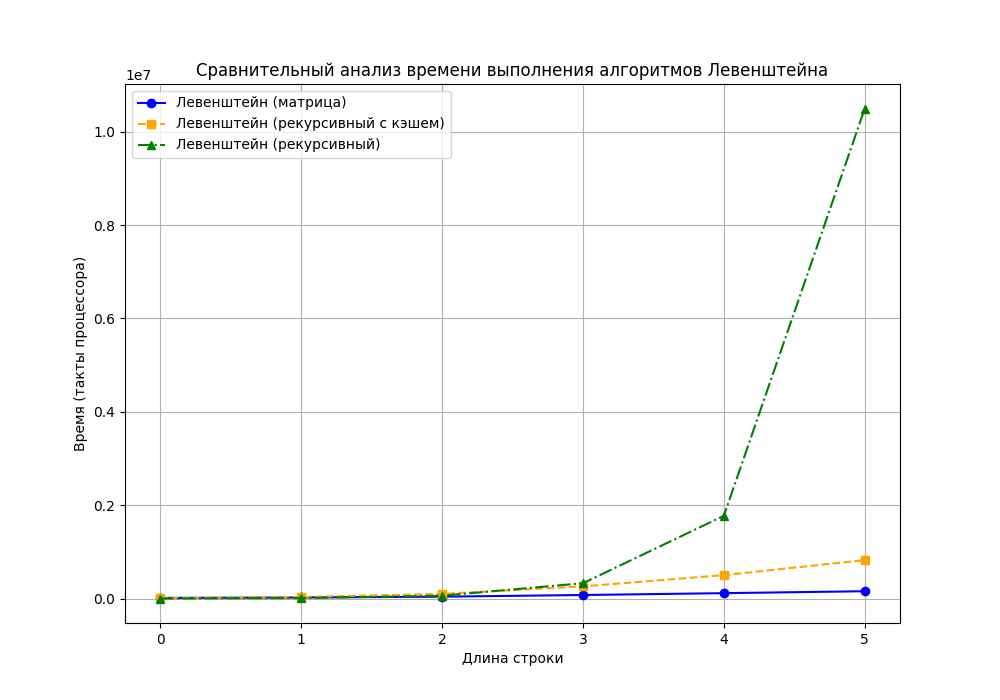
\includegraphics[scale=0.6]{img/all_lev.png}
    \caption{Сравнение времени всех реализаций алгоритмов нахождения расстояний Левенштейна.}
    \label{fig:all_lev}
\end{figure}

В результате тестирования на рисунке~\ref{fig:all_lev} рекурсивный алгоритм Левенштейна оказался наименее эффективным по времени выполнения, в то время как нерекурсивный алгоритм показал наилучшие результаты. Далее приведены графики сравнения оставшихся алгоритмов на большей длине строк. 

\begin{figure}[h]
    \centering
    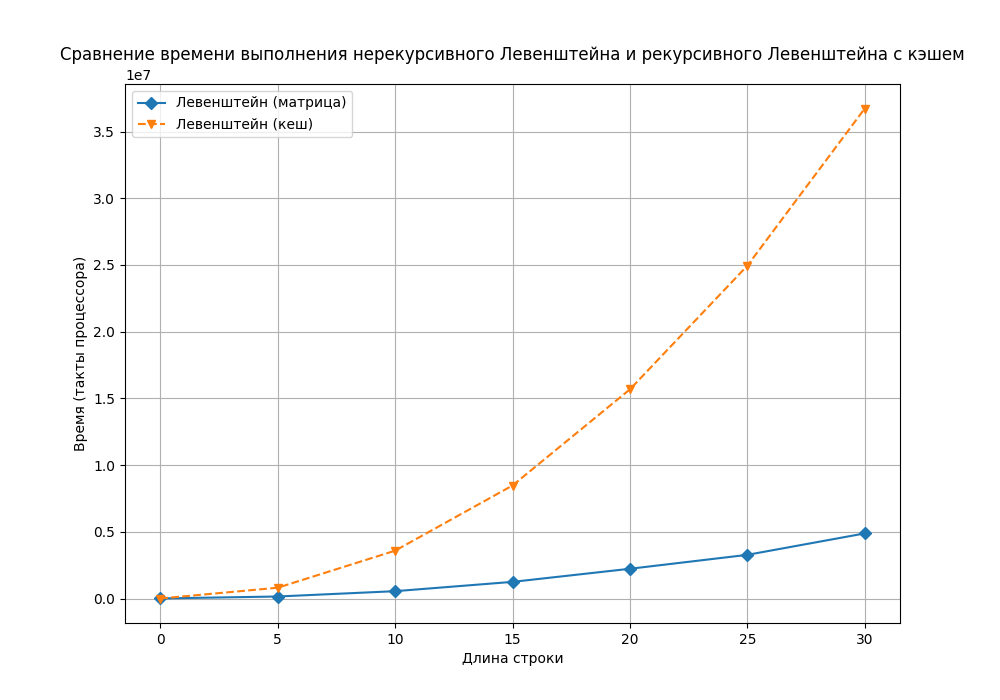
\includegraphics[scale=0.6]{img/lev_2.png}
    \caption{Сравнение нерекурсивного алгоритма Левенштейна и рекурсивного алгоритма Левенштейна с использованием кэша по времени.}
    \label{fig:lev_2}
\end{figure}


\begin{figure}[h]
    \centering
    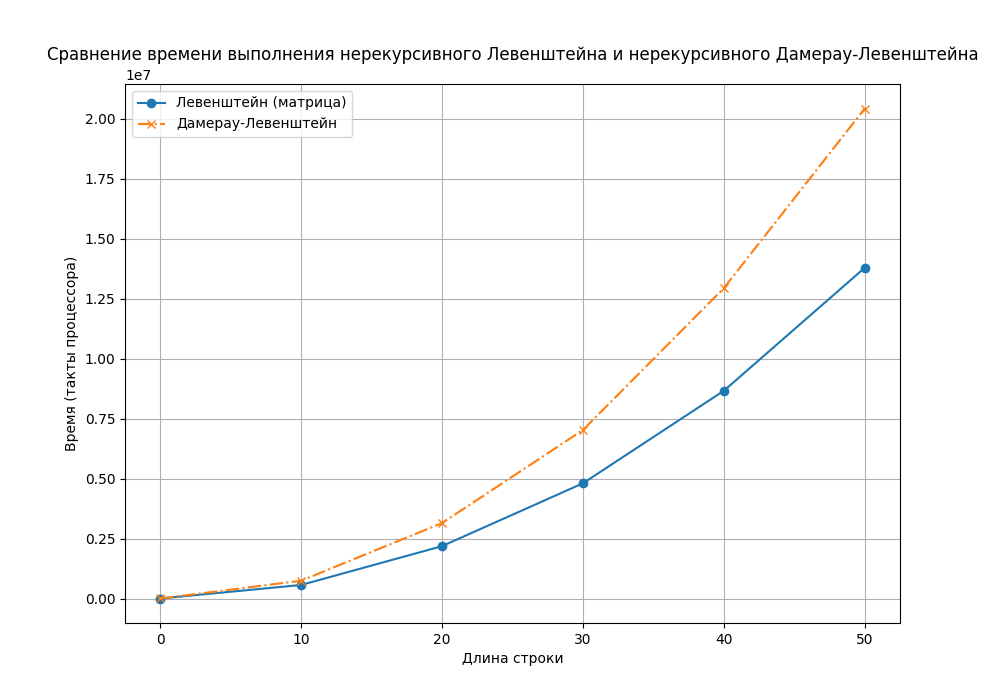
\includegraphics[scale=0.6]{img/dam_lev_3.png} 
    \caption{Сравнение нерекурсивного алгоритма Левенштейна и нерекурсивного алгоритма Дамерау~---~Левенштейна по времени.}
    \label{fig:dam_lev_3}
\end{figure}
\clearpage


\section{Сравнительный анализ использования \newline памяти алгоритмами}
\subsection{Нерекурсивные алгоритмы}
Нерекурсивные алгоритмы нахождения расстояния \texttt{Левенштейна}~\cite{bib4} и Дамерау~---~Левенштейна имеют одинаковые затраты по памяти, так как оба используют матрицу для хранения промежуточных результатов.
В реализации \texttt{levenstein\_matrix} и \texttt{damerau\_levenstein\_matrix} память необходима для создания матрицы, размер которой определяется длинами строк \(n\) и \(m\). Каждая ячейка матрицы содержит целочисленное значение, и общий объем памяти, необходимый для её хранения, пропорционален \((n+1) \times (m+1)\), где \(n\) и \(m\) — длины строк.

Кроме хранения значений матрицы, связанных с операциями вставки, удаления, замены и перестановки символов, используются дополнительные переменные.

Затраты памяти для нерекурсивных алгоритмов:
\[
M_{\text{iter}} = (n+1) \times (m+1) \times \text{size(int)} + (4 \times \text{size(int)})
\]
где:
\begin{itemize}
    \item[--] \(n\) и \(m\) — длины строк;
    \item[--] \(\text{size(int)}\) — объем памяти для хранения одного целочисленного значения;
    \item[--] \(4 \times \text{size(int)}\) — затраты на хранение четырёх переменных, необходимых для операций вставки, удаления, замены и перестановки символов.
\end{itemize}

\subsection{Рекурсивные алгоритмы}

Для рекурсивных алгоритмов, таких как \texttt{levenstein\_recursive}, память расходуется иначе. Каждый раз, когда вызывается рекурсивная функция, она занимает место в стеке вызовов. Глубина стека, которая влияет на использование памяти, зависит от длин строк \(n\) и \(m\). В худшем случае глубина стека равна \(n + m\), это означает, что память будет расходоваться на хранение локальных переменных каждой рекурсивной функции.

Затраты памяти для рекурсивного алгоритма:
\[
M_{\text{rec}} = (n + m) \times \text{size(call stack)} + (3 \times \text{size(int)})
\]
где:
\begin{itemize}
    \item[--] \(\text{size(call stack)}\) — объем памяти, используемой на каждый рекурсивный вызов;
    \item[--] \(3 \times \text{size(int)}\) — затраты на промежуточные переменные для вставки, удаления и замены символов.
\end{itemize}

\subsection{Рекурсивные алгоритмы с кэшированием}
Рекурсивные алгоритмы с кэшированием делают процесс вычисления расстояния Левенштейна более эффективным, уменьшая количество рекурсивных вызовов за счёт сохранения уже вычисленных результатов. Хотя такие алгоритмы требуют больше памяти, чем обычные рекурсивные алгоритмы, из-за необходимости хранения кэша, они ускоряют выполнение за счёт сокращения времени, необходимого для повторного вычисления одних и тех же значений.
\[
M_{\text{rec\_cache}} = (n+1) \times (m+1) \times \text{size(int)} + (n + m) \times \text{size(call stack)} + (3 \times \text{size(int)})
\]

\begin{itemize}
    \item[--] \((n+1) \times (m+1) \times \text{size(int)}\) -- затраты на хранение матрицы;
    
    \item[--] \((n + m) \times \text{size(call stack)}\) -- затраты на стек вызовов. Глубина стека \(n + m\), так как в худшем случае рекурсивный процесс обрабатывает все подстроки длиной \(n\) и \(m\);
    
    \item[--] \(3 \times \text{size(int)}\) -- затраты на промежуточные переменные для вставки, удаления и замены.
\end{itemize}

Таким образом, затраты памяти для рекурсивного алгоритма с кэшированием включают в себя: память на хранение кэша, память для стека рекурсивных вызовов, которая уменьшается благодаря кэшированию, и постоянные затраты на хранение трёх промежуточных переменных.

\section*{Вывод}
Нерекурсивные алгоритмы обеспечивают эффективное использование памяти благодаря сохранению матрицы промежуточных результатов, что позволяет избежать расходов на стек вызовов. Эти алгоритмы предпочтительнее при работе с длинными строками, однако их требования к памяти высоки из-за размеров матрицы.

Рекурсивные алгоритмы без кэширования более экономичны на этапе промежуточных вычислений, но затраты на стек вызовов возрастают с увеличением длины строк, что снижает их эффективность для больших входных данных.

Рекурсивные алгоритмы с кэшированием требуют больше памяти из-за необходимости хранения кэша вычисленных результатов, поэтому нерекурсивные алгоритмы остаются более эффективными в плане использования памяти.


\chapter*{ЗАКЛЮЧЕНИЕ}
\addcontentsline{toc}{chapter}{ЗАКЛЮЧЕНИЕ}
Цель работы достигнута. В ходе выполнения данной лабораторной работы были решены следующие задачи:
\begin{itemize}
    \item[--] исследованы методы расчёта расстояния Левенштейна и Дамерау~---~Левенштейна;
    \item[--] реализован рекурсивный алгоритм для вычисления расстояния Левенштейна;
    \item[--] реализован нерекурсивный алгоритм для вычисления расстояния Левенштейна;
    \item[--] реализован рекурсивный с кэшем алгоритм для вычисления расстояния Левенштейна;
    \item[--] реализован рекурсивный алгоритм для вычисления расстояния Дамерау~---~Левенштейна;
    \item[--] проведено сравнение эффективности этих алгоритмов, исследуя их затраты по затраченному процессорному времени и памяти;
    \item[--] представлены полученные результаты в виде отчёта о выполненной лабораторной работе.
\end{itemize}

Исследования показали, что нерекурсивные алгоритмы быстрее рекурсивных и требуют меньше памяти.

\renewcommand{\bibname}{СПИСОК ИСПОЛЬЗОВАННЫХ ИСТОЧНИКОВ}
\begin{thebibliography}{4}
    \bibitem{bib1}
    Левенштейн, В. И. Бинарные коды, исправляющие удаления, вставки и перестановки. Доклады Академии Наук СССР, 1966, т. 163, с. 845–848.

    \bibitem{bib2}
    Python Software Foundation. Официальная документация языка Python [Электронный ресурс]. -- Режим доступа: \mbox{\url{https://www.python.org/doc/}} (дата обращения: 29.09.2024).
    
    \bibitem{bib3}
    Python Software Foundation. Документация модуля time -- Доступ ко времени и его преобразования [Электронный ресурс]. -- Режим доступа: \mbox{\url{https://docs.python.org/3/library/time.html}} (дата обращения: 29.09.2024).
    
    \bibitem{bib4}
    Чёрненький В. М., Гапанюк Ю. Е. Оценка точности измерительных систем // Вестник МГТУ им. Н.Э. Баумана. Сер. Приборостроение. 2012. № 3. С. 102–110. ISSN 0236-3933.

\end{thebibliography}

%\chapter*{СПИСОК ИСПОЛЬЗОВАННЫХ ИСТОЧНИКОВ}
\addcontentsline{toc}{chapter}{СПИСОК ИСПОЛЬЗОВАННЫХ ИСТОЧНИКОВ}

\end{document}